\documentclass[12pt,a4paper,a4paper]{book}
\usepackage{lmodern}
\usepackage{amssymb,amsmath}
\usepackage{ifxetex,ifluatex}
\usepackage{fixltx2e} % provides \textsubscript
\ifnum 0\ifxetex 1\fi\ifluatex 1\fi=0 % if pdftex
  \usepackage[T1]{fontenc}
  \usepackage[utf8]{inputenc}
\else % if luatex or xelatex
  \ifxetex
    \usepackage{mathspec}
  \else
    \usepackage{fontspec}
  \fi
  \defaultfontfeatures{Ligatures=TeX,Scale=MatchLowercase}
\fi
% use upquote if available, for straight quotes in verbatim environments
\IfFileExists{upquote.sty}{\usepackage{upquote}}{}
% use microtype if available
\IfFileExists{microtype.sty}{%
\usepackage{microtype}
\UseMicrotypeSet[protrusion]{basicmath} % disable protrusion for tt fonts
}{}
\usepackage[margin=2cm]{geometry}
\usepackage{hyperref}
\PassOptionsToPackage{usenames,dvipsnames}{color} % color is loaded by hyperref
\hypersetup{unicode=true,
            pdftitle={Mapping with R},
            pdfauthor={Ernest Guevarra},
            colorlinks=true,
            linkcolor=blue,
            citecolor=blue,
            urlcolor=blue,
            breaklinks=true}
\urlstyle{same}  % don't use monospace font for urls
\usepackage{natbib}
\bibliographystyle{apalike}
\usepackage{color}
\usepackage{fancyvrb}
\newcommand{\VerbBar}{|}
\newcommand{\VERB}{\Verb[commandchars=\\\{\}]}
\DefineVerbatimEnvironment{Highlighting}{Verbatim}{commandchars=\\\{\}}
% Add ',fontsize=\small' for more characters per line
\usepackage{framed}
\definecolor{shadecolor}{RGB}{248,248,248}
\newenvironment{Shaded}{\begin{snugshade}}{\end{snugshade}}
\newcommand{\KeywordTok}[1]{\textcolor[rgb]{0.13,0.29,0.53}{\textbf{#1}}}
\newcommand{\DataTypeTok}[1]{\textcolor[rgb]{0.13,0.29,0.53}{#1}}
\newcommand{\DecValTok}[1]{\textcolor[rgb]{0.00,0.00,0.81}{#1}}
\newcommand{\BaseNTok}[1]{\textcolor[rgb]{0.00,0.00,0.81}{#1}}
\newcommand{\FloatTok}[1]{\textcolor[rgb]{0.00,0.00,0.81}{#1}}
\newcommand{\ConstantTok}[1]{\textcolor[rgb]{0.00,0.00,0.00}{#1}}
\newcommand{\CharTok}[1]{\textcolor[rgb]{0.31,0.60,0.02}{#1}}
\newcommand{\SpecialCharTok}[1]{\textcolor[rgb]{0.00,0.00,0.00}{#1}}
\newcommand{\StringTok}[1]{\textcolor[rgb]{0.31,0.60,0.02}{#1}}
\newcommand{\VerbatimStringTok}[1]{\textcolor[rgb]{0.31,0.60,0.02}{#1}}
\newcommand{\SpecialStringTok}[1]{\textcolor[rgb]{0.31,0.60,0.02}{#1}}
\newcommand{\ImportTok}[1]{#1}
\newcommand{\CommentTok}[1]{\textcolor[rgb]{0.56,0.35,0.01}{\textit{#1}}}
\newcommand{\DocumentationTok}[1]{\textcolor[rgb]{0.56,0.35,0.01}{\textbf{\textit{#1}}}}
\newcommand{\AnnotationTok}[1]{\textcolor[rgb]{0.56,0.35,0.01}{\textbf{\textit{#1}}}}
\newcommand{\CommentVarTok}[1]{\textcolor[rgb]{0.56,0.35,0.01}{\textbf{\textit{#1}}}}
\newcommand{\OtherTok}[1]{\textcolor[rgb]{0.56,0.35,0.01}{#1}}
\newcommand{\FunctionTok}[1]{\textcolor[rgb]{0.00,0.00,0.00}{#1}}
\newcommand{\VariableTok}[1]{\textcolor[rgb]{0.00,0.00,0.00}{#1}}
\newcommand{\ControlFlowTok}[1]{\textcolor[rgb]{0.13,0.29,0.53}{\textbf{#1}}}
\newcommand{\OperatorTok}[1]{\textcolor[rgb]{0.81,0.36,0.00}{\textbf{#1}}}
\newcommand{\BuiltInTok}[1]{#1}
\newcommand{\ExtensionTok}[1]{#1}
\newcommand{\PreprocessorTok}[1]{\textcolor[rgb]{0.56,0.35,0.01}{\textit{#1}}}
\newcommand{\AttributeTok}[1]{\textcolor[rgb]{0.77,0.63,0.00}{#1}}
\newcommand{\RegionMarkerTok}[1]{#1}
\newcommand{\InformationTok}[1]{\textcolor[rgb]{0.56,0.35,0.01}{\textbf{\textit{#1}}}}
\newcommand{\WarningTok}[1]{\textcolor[rgb]{0.56,0.35,0.01}{\textbf{\textit{#1}}}}
\newcommand{\AlertTok}[1]{\textcolor[rgb]{0.94,0.16,0.16}{#1}}
\newcommand{\ErrorTok}[1]{\textcolor[rgb]{0.64,0.00,0.00}{\textbf{#1}}}
\newcommand{\NormalTok}[1]{#1}
\usepackage{longtable,booktabs}
\usepackage{graphicx,grffile}
\makeatletter
\def\maxwidth{\ifdim\Gin@nat@width>\linewidth\linewidth\else\Gin@nat@width\fi}
\def\maxheight{\ifdim\Gin@nat@height>\textheight\textheight\else\Gin@nat@height\fi}
\makeatother
% Scale images if necessary, so that they will not overflow the page
% margins by default, and it is still possible to overwrite the defaults
% using explicit options in \includegraphics[width, height, ...]{}
\setkeys{Gin}{width=\maxwidth,height=\maxheight,keepaspectratio}
\IfFileExists{parskip.sty}{%
\usepackage{parskip}
}{% else
\setlength{\parindent}{0pt}
\setlength{\parskip}{6pt plus 2pt minus 1pt}
}
\setlength{\emergencystretch}{3em}  % prevent overfull lines
\providecommand{\tightlist}{%
  \setlength{\itemsep}{0pt}\setlength{\parskip}{0pt}}
\setcounter{secnumdepth}{5}

%%% Use protect on footnotes to avoid problems with footnotes in titles
\let\rmarkdownfootnote\footnote%
\def\footnote{\protect\rmarkdownfootnote}

%%% Change title format to be more compact
\usepackage{titling}

% Create subtitle command for use in maketitle
\newcommand{\subtitle}[1]{
  \posttitle{
    \begin{center}\large#1\end{center}
    }
}

\setlength{\droptitle}{-2em}

  \title{Mapping with R}
    \pretitle{\vspace{\droptitle}\centering\huge}
  \posttitle{\par}
    \author{Ernest Guevarra}
    \preauthor{\centering\large\emph}
  \postauthor{\par}
      \predate{\centering\large\emph}
  \postdate{\par}
    \date{2018-10-07}

\usepackage{booktabs}
\usepackage[table]{xcolor}
\usepackage{color}
\usepackage{tcolorbox}
\usepackage{float}
\usepackage{setspace}
\usepackage{longtable}
\usepackage{titlesec}
%\usepackage{amsmath}
%\usepackage{mathtools}

\onehalfspacing

%\raggedbottom

\graphicspath{ {icons/} }

\titleformat{\chapter}
  {\normalfont\LARGE\bfseries}{\thechapter}{1em}{}
\titlespacing*{\chapter}{0pt}{3.5ex plus 1ex minus .2ex}{2.3ex plus .2ex}

\newenvironment{rmdremind}
  {\begin{tcolorbox}[width=\textwidth, 
                     colback = {white}, 
                     title = {\textbf{Remember}}, 
                     colbacktitle = lightgray,
                     coltitle = black]
  \begin{includegraphics}[scale = 1]{remind.png}
  \begin{itemize}}
  {\end{itemize}
  \end{includegraphics}
  \end{tcolorbox}}

\newenvironment{rmdnote}
  {\begin{tcolorbox}[width=\textwidth, 
                     colback = {white}, 
                     title = {\textbf{Note}}, 
                     colbacktitle = lightgray,
                     coltitle = black]
  \begin{includegraphics}[scale = 1]{pencil.png}}
  {\end{includegraphics}
  \end{tcolorbox}}
  
\newenvironment{rmdcalc}
  {\begin{tcolorbox}[width=\textwidth, 
                     colback = {white}, 
                     title = {\textbf{Calculations}}, 
                     colbacktitle = lightgray,
                     coltitle = black]
  \begin{includegraphics}[scale = 2]{pencil.png}}
  {\end{includegraphics}
  \end{tcolorbox}}
  
\newenvironment{rmdexercise}
  {\begin{tcolorbox}[width=\textwidth, 
                     colback = {white}, 
                     title = {\textbf{Exercise}}, 
                     colbacktitle = lightgray,
                     coltitle = black]
  \begin{includegraphics}[scale = 1]{exercise.png}}
  {\end{includegraphics}
  \end{tcolorbox}}
  
\newenvironment{rmdbox}
  {\begin{tcolorbox}[width=\textwidth, 
                     colback = {white}, 
                     title = {\textbf{Exercise}}, 
                     colbacktitle = lightgray,
                     coltitle = black]
  \begin{includegraphics}[scale = 1]{pencil.png}}
  {\end{includegraphics}
  \end{tcolorbox}}
  
\newenvironment{rmdinfo}
  {\begin{tcolorbox}[width=\textwidth, 
                     colback = {white}, 
                     title = {\textbf{Info}}, 
                     colbacktitle = lightgray,
                     coltitle = black]
  \begin{includegraphics}[scale = 1]{info.png}}
  {\end{includegraphics}
  \end{tcolorbox}}  
  
\newenvironment{rmdwarning}
  {\begin{tcolorbox}[width=\textwidth, 
                     colback = {white}, 
                     title = {\textbf{Warning}}, 
                     colbacktitle = lightgray,
                     coltitle = black]
  \begin{includegraphics}[scale = 1]{warning.png}}
  {\end{includegraphics}
  \end{tcolorbox}}

\newenvironment{rmdcaution}
  {\begin{tcolorbox}[width=\textwidth, 
                     colback = {white}, 
                     title = {\textbf{Caution}}, 
                     colbacktitle = lightgray,
                     coltitle = black]
  \begin{includegraphics}[scale = 1]{warning.png}}
  {\end{includegraphics}
  \end{tcolorbox}}

\newenvironment{rmddownload}
  {\begin{tcolorbox}[width=\textwidth, 
                     colback = {white}, 
                     title = {\textbf{Download}}, 
                     colbacktitle = lightgray,
                     coltitle = black]
  \begin{includegraphics}[scale = 1]{download.png}}
  {\end{includegraphics}
  \end{tcolorbox}}

\usepackage{amsthm}
\newtheorem{theorem}{Theorem}[chapter]
\newtheorem{lemma}{Lemma}[chapter]
\theoremstyle{definition}
\newtheorem{definition}{Definition}[chapter]
\newtheorem{corollary}{Corollary}[chapter]
\newtheorem{proposition}{Proposition}[chapter]
\theoremstyle{definition}
\newtheorem{example}{Example}[chapter]
\theoremstyle{definition}
\newtheorem{exercise}{Exercise}[chapter]
\theoremstyle{remark}
\newtheorem*{remark}{Remark}
\newtheorem*{solution}{Solution}
\begin{document}
\maketitle

{
\hypersetup{linkcolor=black}
\setcounter{tocdepth}{1}
\tableofcontents
}
\listoftables
\listoffigures
\hypertarget{short-course-on-the-use-of-r-for-the-mapping-requirements-of-s3m}{%
\chapter*{Short course on the use of R for the mapping requirements of
S3M}\label{short-course-on-the-use-of-r-for-the-mapping-requirements-of-s3m}}
\addcontentsline{toc}{chapter}{Short course on the use of R for the
mapping requirements of S3M}

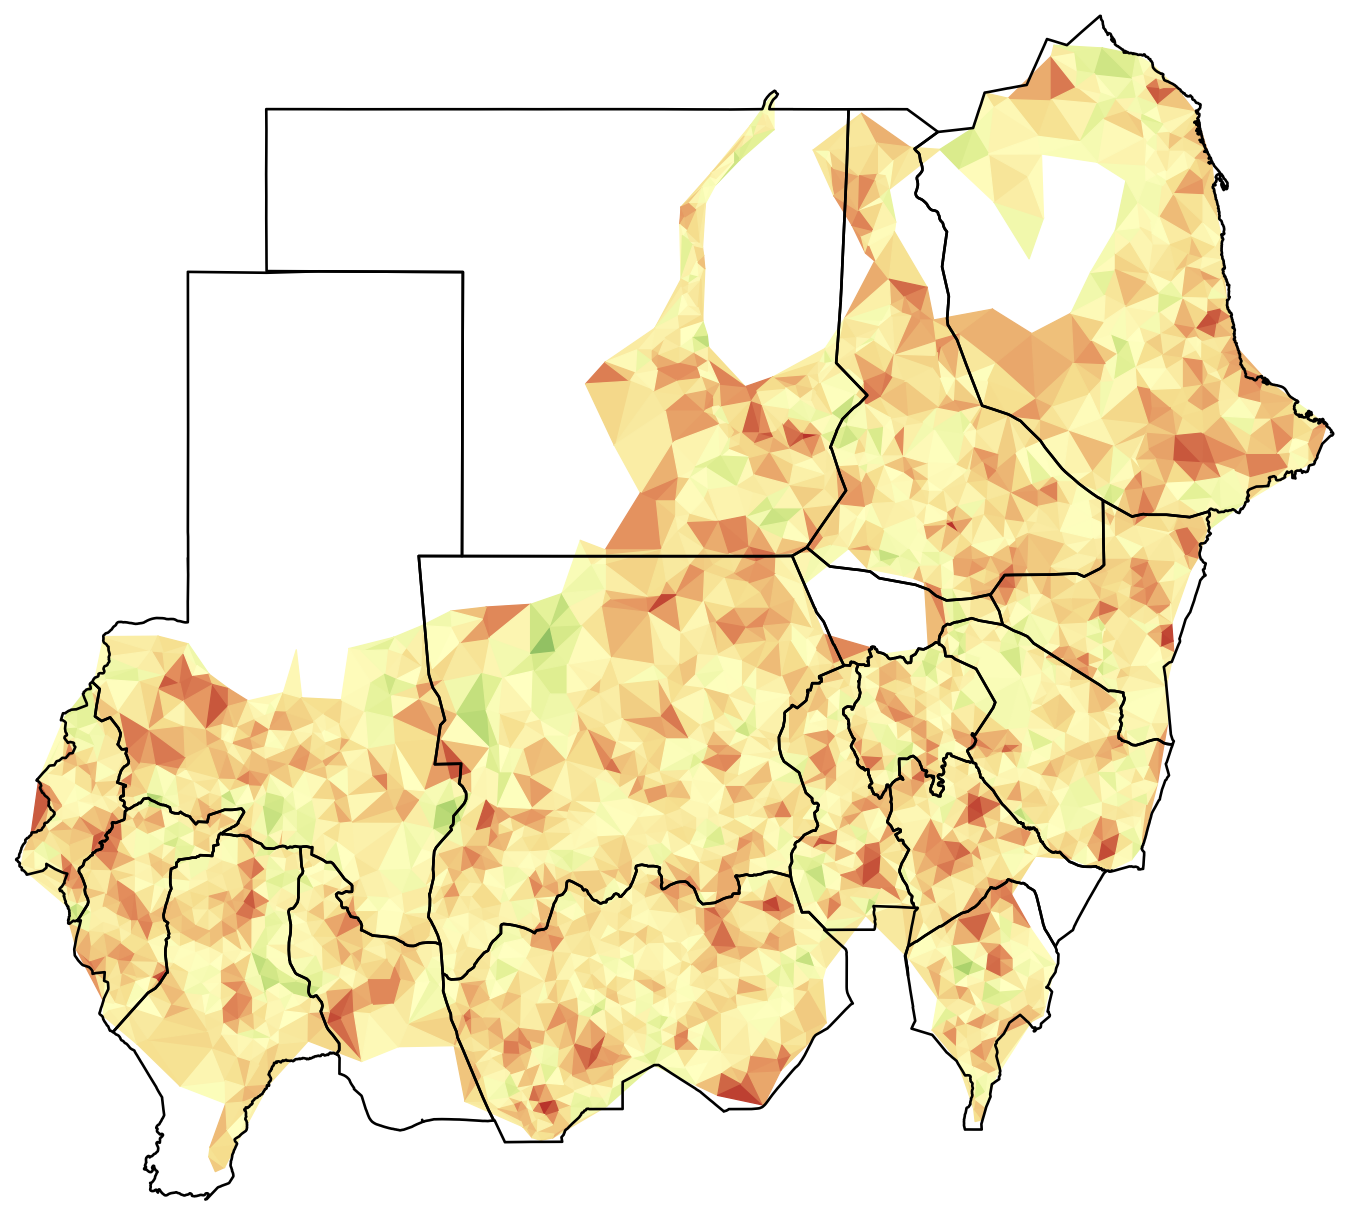
\includegraphics{figures/sudanMapTriSim.png}

\hypertarget{exercise1}{%
\chapter{Retrieving map data in R}\label{exercise1}}

In this exercise we will use \textbf{R} to read a \textbf{shapefile}
dataset and get oriented with the structure and features of a
\textbf{shapefile} dataset. The aim of the exercise is for you to become
familiar with the use of R in handling \textbf{shapefile} datasets.

By this time, you have already learned how to issue a command to
retrieve a standard or typical dataset using the \texttt{read.table()}
function

For this exercise, we will use the \texttt{readOGR()} function provided
by the \texttt{rgdal} package to retrieve \textbf{shapefile} dateset.

First, we need to install and load the \texttt{rgdal} package.

~

\begin{Shaded}
\begin{Highlighting}[]
\KeywordTok{install.packages}\NormalTok{(“rgdal”)}
\KeywordTok{library}\NormalTok{(rgdal)}
\end{Highlighting}
\end{Shaded}

~

We can now try to read the Sudan \textbf{shapefile}. To do this however,
we need to have an orientation on what \textbf{shapefiles} are.

A \textbf{shapefile} is a digital vector storage format for storing
geometric location and associated attribute information. This format
lacks the capacity to store topological information. The
\textbf{shapefile} format was initially developed for proprietary use
with ArcView GIS version 2 in the early 1990s. It is now possible to
read and write \textbf{shapefiles} using a variety of programs including
data analysis software such as \textbf{R}.

\textbf{Shapefiles} are simple because they store the primitive
geometric data types of points, lines, and polygons. They are of limited
use without any attributes to specify what they represent. Therefore, a
table of records will store properties/attributes for each primitive
shape in the \textbf{shapefile}. Shapes (points/lines/polygons) together
with data attributes can create infinitely many representations about
geographic data. Representation provides the ability for powerful and
accurate computations.

While the term ``shapefile'' is quite common, a \textbf{shapefile} is
actually a set of several files. Three individual files are mandatory to
store the core data that comprise a \textbf{shapefile}:

\begin{itemize}
\tightlist
\item
  .shp
\item
  .shx
\item
  .dbf
\end{itemize}

The actual \textbf{shapefile} relates specifically to \texttt{.shp}
files but alone is incomplete for distribution, as the other supporting
files are required.

With this knowledge of \textbf{shapefiles}, let us now take a look at
the Sudan \textbf{shapefiles} dataset.

The Sudan \textbf{shapefiles} dataset contains the following
\textbf{shapefiles}:

~

\begin{longtable}[]{@{}lll@{}}
\caption{\label{tab:table1} Sudan shapefiles structure}\tabularnewline
\toprule
\begin{minipage}[b]{0.23\columnwidth}\raggedright
\textbf{Directory name}\strut
\end{minipage} & \begin{minipage}[b]{0.23\columnwidth}\raggedright
\textbf{Directory files}\strut
\end{minipage} & \begin{minipage}[b]{0.45\columnwidth}\raggedright
\textbf{Description}\strut
\end{minipage}\tabularnewline
\midrule
\endfirsthead
\toprule
\begin{minipage}[b]{0.23\columnwidth}\raggedright
\textbf{Directory name}\strut
\end{minipage} & \begin{minipage}[b]{0.23\columnwidth}\raggedright
\textbf{Directory files}\strut
\end{minipage} & \begin{minipage}[b]{0.45\columnwidth}\raggedright
\textbf{Description}\strut
\end{minipage}\tabularnewline
\midrule
\endhead
\begin{minipage}[t]{0.23\columnwidth}\raggedright
sudan01\strut
\end{minipage} & \begin{minipage}[t]{0.23\columnwidth}\raggedright
sudan01.shp sudan01.shx sudan01.dbf sudan01.prj sudan01.qpj\strut
\end{minipage} & \begin{minipage}[t]{0.45\columnwidth}\raggedright
Polygon shapefile of Sudan up to state administrative level\strut
\end{minipage}\tabularnewline
\begin{minipage}[t]{0.23\columnwidth}\raggedright
sudan02\strut
\end{minipage} & \begin{minipage}[t]{0.23\columnwidth}\raggedright
sudan02.shp sudan02.shx sudan02.dbf sudan02.prj sudan02.qpj\strut
\end{minipage} & \begin{minipage}[t]{0.45\columnwidth}\raggedright
Polygon shapefile of Sudan up to locality administrative level\strut
\end{minipage}\tabularnewline
\begin{minipage}[t]{0.23\columnwidth}\raggedright
grid12poly\strut
\end{minipage} & \begin{minipage}[t]{0.23\columnwidth}\raggedright
grid12poly.shp grid12poly.shx grid12poly.dbf grid12poly.prj
grid12poly.qpj\strut
\end{minipage} & \begin{minipage}[t]{0.45\columnwidth}\raggedright
Polygon shapefile of rectangular grid at d = 12km\strut
\end{minipage}\tabularnewline
\begin{minipage}[t]{0.23\columnwidth}\raggedright
grid12kmSudan\strut
\end{minipage} & \begin{minipage}[t]{0.23\columnwidth}\raggedright
grid12kmSudan.shp grid12kmSudan.shx grid12kmSudan.dbf grid12kmSudan.prj
grid12kmSudan.qpj\strut
\end{minipage} & \begin{minipage}[t]{0.45\columnwidth}\raggedright
Line shapefile of rectangular grid at d = 12km\strut
\end{minipage}\tabularnewline
\bottomrule
\end{longtable}

~

We can now retrieve these shapefile datasets and create an object for
each one using the \texttt{readOGR()} function from the \texttt{rgdal}
package.

~

\begin{Shaded}
\begin{Highlighting}[]
\NormalTok{sudan01 <-}\StringTok{ }\KeywordTok{readOGR}\NormalTok{(}\DataTypeTok{dsn =} \StringTok{"maps"}\NormalTok{, }\DataTypeTok{layer =} \StringTok{"sudan01"}\NormalTok{)}
\CommentTok{#> OGR data source with driver: ESRI Shapefile }
\CommentTok{#> Source: "/Users/ernest/Documents/GitHub/map-r/maps", layer: "sudan01"}
\CommentTok{#> with 18 features}
\CommentTok{#> It has 8 fields}

\NormalTok{sudan02 <-}\StringTok{ }\KeywordTok{readOGR}\NormalTok{(}\DataTypeTok{dsn =} \StringTok{"maps"}\NormalTok{, }\DataTypeTok{layer =} \StringTok{"sudan02"}\NormalTok{)}
\CommentTok{#> OGR data source with driver: ESRI Shapefile }
\CommentTok{#> Source: "/Users/ernest/Documents/GitHub/map-r/maps", layer: "sudan02"}
\CommentTok{#> with 169 features}
\CommentTok{#> It has 15 fields}

\NormalTok{grid12poly <-}\StringTok{ }\KeywordTok{readOGR}\NormalTok{(}\DataTypeTok{dsn =} \StringTok{"maps"}\NormalTok{, }\DataTypeTok{layer =} \StringTok{"grid12poly"}\NormalTok{)}
\CommentTok{#> OGR data source with driver: ESRI Shapefile }
\CommentTok{#> Source: "/Users/ernest/Documents/GitHub/map-r/maps", layer: "grid12poly"}
\CommentTok{#> with 13950 features}
\CommentTok{#> It has 5 fields}
\CommentTok{#> Integer64 fields read as strings:  ID}

\NormalTok{grid12kmSudan <-}\StringTok{ }\KeywordTok{readOGR}\NormalTok{(}\DataTypeTok{dsn =} \StringTok{"maps"}\NormalTok{, }\DataTypeTok{layer =} \StringTok{"grid12kmSudan"}\NormalTok{)}
\CommentTok{#> OGR data source with driver: ESRI Shapefile }
\CommentTok{#> Source: "/Users/ernest/Documents/GitHub/map-r/maps", layer: "grid12kmSudan"}
\CommentTok{#> with 245 features}
\CommentTok{#> It has 2 fields}
\CommentTok{#> Integer64 fields read as strings:  ID}
\end{Highlighting}
\end{Shaded}

~

This series of commands illustrates key things about the way shapefile
data can be read and handled in \textbf{R}.

First is that the retrieval of \textbf{shapefile} datasets follows a
very similar syntax as that of other standard datasets but just using
the \texttt{readOGR()} function. The same principles apply including
ensuring that you specify the corresponding directory in which your
\textbf{shapefiles} are stored.

Now that we have stored the various shapefile data into objects, we can
now explore and get ourselves oriented to the structure and features of
a \textbf{shapefile} data object. We will do this using standard / basic
functions in \textbf{R} that you have learned already in the previous
training.

First, let us learn the class of a \textbf{shapefile} data object. We
can find this out using the same function that you are familiar with
already and have used previously the \texttt{class()} function.

~

\begin{Shaded}
\begin{Highlighting}[]
\KeywordTok{class}\NormalTok{(sudan01)}
\end{Highlighting}
\end{Shaded}

~

This command gives the following output:

~

\begin{verbatim}
#> [1] "SpatialPolygonsDataFrame"
#> attr(,"package")
#> [1] "sp"
\end{verbatim}

~

This tells us that the \texttt{sudan01} object is of class
\texttt{SpatialPolygonsDataFrame}. It also tells us that this is a
special class specific to the \texttt{sp} package.

The \texttt{sp} package provides classes and methods for spatial data.
The classes document where the spatial location information resides, for
2D or 3D data. Utility functions are provided, e.g.~for plotting data as
maps, spatial selection, as well as methods for retrieving coordinates,
for subsetting, print, summary, etc.

If you check for the class of the other \textbf{shapefile} objects
you've created, you will see that all of them are of the same
\texttt{SpatialPolygonsDataFrame} class except for
\texttt{grid12kmSudan}. Checking for the class of \texttt{grid12kmSudan}
revealed the following:

~

\begin{Shaded}
\begin{Highlighting}[]
\KeywordTok{class}\NormalTok{(grid12kmSudan)}
\CommentTok{#> [1] "SpatialLinesDataFrame"}
\CommentTok{#> attr(,"package")}
\CommentTok{#> [1] "sp"}
\end{Highlighting}
\end{Shaded}

~

This tells us that the \texttt{grid12kmSudan} objects is of class
\texttt{SpatialLinesDataFrame}.

You are now getting introduced to two of the most common shapes of a
\textbf{shapefile}: \emph{polygons} and \emph{lines}.

A \emph{polygon} consists of one or more rings. A ring is a connected
sequence of four or more points that form a closed,
non-self-intersecting loop. A \emph{polygon} may contain multiple outer
rings. The order of vertices or orientation for a ring indicates which
side of the ring is the interior of the \emph{polygon}. The
neighbourhood to the right of an observer walking along the ring in
vertex order is the neighbourhood inside the \emph{polygon}. Vertices of
rings defining holes in \emph{polygons} are in a counterclockwise
direction. Vertices for a single, ringed \emph{polygon} are, therefore,
always in clockwise order. The rings of a \emph{polygon} are referred to
as its parts.

A \emph{line} is an ordered set of vertices that consists of one or more
parts. A part is a connected sequence of two or more points. Parts may
or may not be connected to one another. Parts may or may not intersect
one another.

One of the other shapes that \textbf{shapefiles} take or represent is
\emph{points}.

A \emph{point} consists of a pair of double-precision coordinates in the
order \texttt{x}, \texttt{y}.

Because of this simple property of a \emph{point} \textbf{shapefile}
(i.e.~a basic set of \texttt{x} and \texttt{y} coordinates), the use of
\textbf{shapefile} format to store the \emph{point} shape is not
commonly used. The \texttt{x} and \texttt{y} coordinates for
\emph{points} can be contained or stored in other more basic formats
such as CSV.

For example, the dataset that contains the \texttt{x} and \texttt{y}
coordinates of all the known villages in Sudan is named
\texttt{settlementsSudan.csv}. If we create an object called villages
for this dataset

~

\begin{Shaded}
\begin{Highlighting}[]
\NormalTok{villages <-}\StringTok{ }\KeywordTok{read.csv}\NormalTok{(}\StringTok{"maps/settlementsSudan.csv"}\NormalTok{, }\DataTypeTok{header =} \OtherTok{TRUE}\NormalTok{, }\DataTypeTok{sep =} \StringTok{","}\NormalTok{)}
\end{Highlighting}
\end{Shaded}

~

and use the \texttt{head()} function to view the first 10 rows of this
dataset

~

\begin{Shaded}
\begin{Highlighting}[]
\KeywordTok{head}\NormalTok{(villages, }\DecValTok{10}\NormalTok{)}
\end{Highlighting}
\end{Shaded}

~

we get:

~

\begin{verbatim}
#>    ID      Village Pop     Source      State Locality        X        Y
#> 1   1        Kosti         Georef White Nile    Kosti 32.66751 13.14846
#> 2   2     Tandalti     Calculated White Nile    Kosti 31.86393 13.00969
#> 3   3    Qawz kobi            GPS White Nile    Kosti 32.35000 13.60000
#> 4   4    Karjuggle            GPS White Nile    Kosti 32.38333 13.46667
#> 5   5   Idd maktuf            GPS White Nile    Kosti 32.28333 13.50000
#> 6   6       Maryam            GPS White Nile    Kosti 32.55000 13.46667
#> 7   7 Qawz nyaneir            GPS White Nile    Kosti 32.28333 13.60000
#> 8   8       Salogi            GPS White Nile    Kosti 32.45000 13.15000
#> 9   9      Sulayah            GPS White Nile    Kosti 32.25000 13.26667
#> 10 10      Seleima     Calculated White Nile    Kosti 32.05833 13.00833
#>    Remarks
#> 1         
#> 2         
#> 3         
#> 4         
#> 5         
#> 6         
#> 7         
#> 8         
#> 9         
#> 10
\end{verbatim}

~

As you will notice here, the villages object contains information on the
\texttt{x} and \texttt{y} coordinates of each of the villages in Sudan.
So, whilst this dataset is not a \textbf{shapefile} (it is a basic data
frame), it has information and a structure that is comparable to a point
\textbf{shapefile} as defined above.

In the succeeding exercises, this similarity of a \emph{point}
\textbf{shapefile} and a standard data frame containing \texttt{x} and
\texttt{y} coordinates of \emph{points} will be further discussed and
illuminated.

This knowledge on classes and shapes of \textbf{shapefiles} is an
important learning particularly when performing functions to handle or
manipulate different \textbf{shapefile} objects. The general principle
is that functions or operations between two or more \textbf{shapefile}
objects require these objects to be of the same class or family of
classes. Also, the shapes defined by the \textbf{shapefile} object
determine the way the \textbf{shapefile} data is structured which in
turn determine how these objects can and should be handled or
manipulated in \textbf{R}. These principles will be further illuminated
in the succeeding exercises.

After learning about the class of \textbf{shapefile} objects, we now
learn about the structure of these objects. We are able to appreciate
the structure of a \textbf{shapefile} object by using the function
\texttt{str()}.

~

\begin{Shaded}
\begin{Highlighting}[]
\KeywordTok{str}\NormalTok{(sudan01)}
\end{Highlighting}
\end{Shaded}

~

The output of this command is:

~

\begin{verbatim}
#> Formal class 'SpatialPolygonsDataFrame' [package "sp"] with 5 slots
#>   ..@ data       :'data.frame':  18 obs. of  8 variables:
#>   .. ..$ State     : chr [1:18] "West Darfur" "Central Darfur" "North Darfur" "East Darfur" ...
#>   .. ..$ Old_state : chr [1:18] "West Darfur" "West Darfur" "North Darfur" "South Darfur" ...
#>   .. ..$ New_State : chr [1:18] "West Darfur" "Central Darfur" "North Darfur" "East Darfur" ...
#>   .. ..$ STATE_1   : chr [1:18] NA NA NA NA ...
#>   .. ..$ STATEAR   : chr [1:18] NA NA NA NA ...
#>   .. ..$ Source    : chr [1:18] NA NA NA NA ...
#>   .. ..$ STATE_CODE: chr [1:18] NA NA NA NA ...
#>   .. ..$ ISO_CODE  : chr [1:18] NA NA NA NA ...
#>   ..@ polygons   :List of 18
#>   .. ..$ :Formal class 'Polygons' [package "sp"] with 5 slots
#>   .. .. .. ..@ Polygons :List of 1
#>   .. .. .. .. ..$ :Formal class 'Polygon' [package "sp"] with 5 slots
#>   .. .. .. .. .. .. ..@ labpt  : num [1:2] 22.6 13.5
#>   .. .. .. .. .. .. ..@ area   : num 1.86
#>   .. .. .. .. .. .. ..@ hole   : logi FALSE
#>   .. .. .. .. .. .. ..@ ringDir: int 1
#>   .. .. .. .. .. .. ..@ coords : num [1:981, 1:2] 22.1 22.1 22.1 22.2 22.2 ...
#>   .. .. .. ..@ plotOrder: int 1
#>   .. .. .. ..@ labpt    : num [1:2] 22.6 13.5
#>   .. .. .. ..@ ID       : chr "0"
#>   .. .. .. ..@ area     : num 1.86
#>   .. ..$ :Formal class 'Polygons' [package "sp"] with 5 slots
#>   .. .. .. ..@ Polygons :List of 1
#>   .. .. .. .. ..$ :Formal class 'Polygon' [package "sp"] with 5 slots
#>   .. .. .. .. .. .. ..@ labpt  : num [1:2] 23.4 12.3
#>   .. .. .. .. .. .. ..@ area   : num 2.75
#>   .. .. .. .. .. .. ..@ hole   : logi FALSE
#>   .. .. .. .. .. .. ..@ ringDir: int 1
#>   .. .. .. .. .. .. ..@ coords : num [1:463, 1:2] 23.6 23.6 23.6 23.6 23.7 ...
#>   .. .. .. ..@ plotOrder: int 1
#>   .. .. .. ..@ labpt    : num [1:2] 23.4 12.3
#>   .. .. .. ..@ ID       : chr "1"
#>   .. .. .. ..@ area     : num 2.75
#>   .. ..$ :Formal class 'Polygons' [package "sp"] with 5 slots
#>   .. .. .. ..@ Polygons :List of 1
#>   .. .. .. .. ..$ :Formal class 'Polygon' [package "sp"] with 5 slots
#>   .. .. .. .. .. .. ..@ labpt  : num [1:2] 25.6 16.2
#>   .. .. .. .. .. .. ..@ area   : num 26.7
#>   .. .. .. .. .. .. ..@ hole   : logi FALSE
#>   .. .. .. .. .. .. ..@ ringDir: int 1
#>   .. .. .. .. .. .. ..@ coords : num [1:669, 1:2] 27.5 27.5 27.2 27.1 26.9 ...
#>   .. .. .. ..@ plotOrder: int 1
#>   .. .. .. ..@ labpt    : num [1:2] 25.6 16.2
#>   .. .. .. ..@ ID       : chr "2"
#>   .. .. .. ..@ area     : num 26.7
#>   .. ..$ :Formal class 'Polygons' [package "sp"] with 5 slots
#>   .. .. .. ..@ Polygons :List of 1
#>   .. .. .. .. ..$ :Formal class 'Polygon' [package "sp"] with 5 slots
#>   .. .. .. .. .. .. ..@ labpt  : num [1:2] 26.5 11
#>   .. .. .. .. .. .. ..@ area   : num 4.44
#>   .. .. .. .. .. .. ..@ hole   : logi FALSE
#>   .. .. .. .. .. .. ..@ ringDir: int 1
#>   .. .. .. .. .. .. ..@ coords : num [1:932, 1:2] 25.5 25.6 25.6 25.6 25.6 ...
#>   .. .. .. ..@ plotOrder: int 1
#>   .. .. .. ..@ labpt    : num [1:2] 26.5 11
#>   .. .. .. ..@ ID       : chr "3"
#>   .. .. .. ..@ area     : num 4.44
#>   .. ..$ :Formal class 'Polygons' [package "sp"] with 5 slots
#>   .. .. .. ..@ Polygons :List of 1
#>   .. .. .. .. ..$ :Formal class 'Polygon' [package "sp"] with 5 slots
#>   .. .. .. .. .. .. ..@ labpt  : num [1:2] 24.4 11
#>   .. .. .. .. .. .. ..@ area   : num 6.91
#>   .. .. .. .. .. .. ..@ hole   : logi FALSE
#>   .. .. .. .. .. .. ..@ ringDir: int 1
#>   .. .. .. .. .. .. ..@ coords : num [1:1896, 1:2] 24.4 24.4 24.4 24.4 24.4 ...
#>   .. .. .. ..@ plotOrder: int 1
#>   .. .. .. ..@ labpt    : num [1:2] 24.4 11
#>   .. .. .. ..@ ID       : chr "4"
#>   .. .. .. ..@ area     : num 6.91
#>   .. ..$ :Formal class 'Polygons' [package "sp"] with 5 slots
#>   .. .. .. ..@ Polygons :List of 1
#>   .. .. .. .. ..$ :Formal class 'Polygon' [package "sp"] with 5 slots
#>   .. .. .. .. .. .. ..@ labpt  : num [1:2] 33.3 14.6
#>   .. .. .. .. .. .. ..@ area   : num 2.28
#>   .. .. .. .. .. .. ..@ hole   : logi FALSE
#>   .. .. .. .. .. .. ..@ ringDir: int 1
#>   .. .. .. .. .. .. ..@ coords : num [1:490, 1:2] 33.6 33.6 33.6 33.6 33.6 ...
#>   .. .. .. ..@ plotOrder: int 1
#>   .. .. .. ..@ labpt    : num [1:2] 33.3 14.6
#>   .. .. .. ..@ ID       : chr "5"
#>   .. .. .. ..@ area     : num 2.28
#>   .. ..$ :Formal class 'Polygons' [package "sp"] with 5 slots
#>   .. .. .. ..@ Polygons :List of 1
#>   .. .. .. .. ..$ :Formal class 'Polygon' [package "sp"] with 5 slots
#>   .. .. .. .. .. .. ..@ labpt  : num [1:2] 34.1 11.3
#>   .. .. .. .. .. .. ..@ area   : num 3.16
#>   .. .. .. .. .. .. ..@ hole   : logi FALSE
#>   .. .. .. .. .. .. ..@ ringDir: int 1
#>   .. .. .. .. .. .. ..@ coords : num [1:406, 1:2] 34.5 34.5 34.5 34.5 34.5 ...
#>   .. .. .. ..@ plotOrder: int 1
#>   .. .. .. ..@ labpt    : num [1:2] 34.1 11.3
#>   .. .. .. ..@ ID       : chr "6"
#>   .. .. .. ..@ area     : num 3.16
#>   .. ..$ :Formal class 'Polygons' [package "sp"] with 5 slots
#>   .. .. .. ..@ Polygons :List of 1
#>   .. .. .. .. ..$ :Formal class 'Polygon' [package "sp"] with 5 slots
#>   .. .. .. .. .. .. ..@ labpt  : num [1:2] 35.1 14.2
#>   .. .. .. .. .. .. ..@ area   : num 4.99
#>   .. .. .. .. .. .. ..@ hole   : logi FALSE
#>   .. .. .. .. .. .. ..@ ringDir: int 1
#>   .. .. .. .. .. .. ..@ coords : num [1:505, 1:2] 34.2 34.3 34.4 34.4 34.5 ...
#>   .. .. .. ..@ plotOrder: int 1
#>   .. .. .. ..@ labpt    : num [1:2] 35.1 14.2
#>   .. .. .. ..@ ID       : chr "7"
#>   .. .. .. ..@ area     : num 4.99
#>   .. ..$ :Formal class 'Polygons' [package "sp"] with 5 slots
#>   .. .. .. ..@ Polygons :List of 1
#>   .. .. .. .. ..$ :Formal class 'Polygon' [package "sp"] with 5 slots
#>   .. .. .. .. .. .. ..@ labpt  : num [1:2] 35.9 15.8
#>   .. .. .. .. .. .. ..@ area   : num 4.1
#>   .. .. .. .. .. .. ..@ hole   : logi FALSE
#>   .. .. .. .. .. .. ..@ ringDir: int 1
#>   .. .. .. .. .. .. ..@ coords : num [1:294, 1:2] 35.7 36 36.1 36.2 36.2 ...
#>   .. .. .. ..@ plotOrder: int 1
#>   .. .. .. ..@ labpt    : num [1:2] 35.9 15.8
#>   .. .. .. ..@ ID       : chr "8"
#>   .. .. .. ..@ area     : num 4.1
#>   .. ..$ :Formal class 'Polygons' [package "sp"] with 5 slots
#>   .. .. .. ..@ Polygons :List of 1
#>   .. .. .. .. ..$ :Formal class 'Polygon' [package "sp"] with 5 slots
#>   .. .. .. .. .. .. ..@ labpt  : num [1:2] 32.8 15.9
#>   .. .. .. .. .. .. ..@ area   : num 1.79
#>   .. .. .. .. .. .. ..@ hole   : logi FALSE
#>   .. .. .. .. .. .. ..@ ringDir: int 1
#>   .. .. .. .. .. .. ..@ coords : num [1:198, 1:2] 33.5 33.7 34 34 34 ...
#>   .. .. .. ..@ plotOrder: int 1
#>   .. .. .. ..@ labpt    : num [1:2] 32.8 15.9
#>   .. .. .. ..@ ID       : chr "9"
#>   .. .. .. ..@ area     : num 1.79
#>   .. ..$ :Formal class 'Polygons' [package "sp"] with 5 slots
#>   .. .. .. ..@ Polygons :List of 1
#>   .. .. .. .. ..$ :Formal class 'Polygon' [package "sp"] with 5 slots
#>   .. .. .. .. .. .. ..@ labpt  : num [1:2] 33.5 18.3
#>   .. .. .. .. .. .. ..@ area   : num 11.1
#>   .. .. .. .. .. .. ..@ hole   : logi FALSE
#>   .. .. .. .. .. .. ..@ ringDir: int 1
#>   .. .. .. .. .. .. ..@ coords : num [1:226, 1:2] 35.6 35.4 35.4 35.3 35.3 ...
#>   .. .. .. ..@ plotOrder: int 1
#>   .. .. .. ..@ labpt    : num [1:2] 33.5 18.3
#>   .. .. .. ..@ ID       : chr "10"
#>   .. .. .. ..@ area     : num 11.1
#>   .. ..$ :Formal class 'Polygons' [package "sp"] with 5 slots
#>   .. .. .. ..@ Polygons :List of 1
#>   .. .. .. .. ..$ :Formal class 'Polygon' [package "sp"] with 5 slots
#>   .. .. .. .. .. .. ..@ labpt  : num [1:2] 29.3 19.6
#>   .. .. .. .. .. .. ..@ area   : num 31.4
#>   .. .. .. .. .. .. ..@ hole   : logi FALSE
#>   .. .. .. .. .. .. ..@ ringDir: int 1
#>   .. .. .. .. .. .. ..@ coords : num [1:117, 1:2] 31.7 32.1 32.1 32.4 32.4 ...
#>   .. .. .. ..@ plotOrder: int 1
#>   .. .. .. ..@ labpt    : num [1:2] 29.3 19.6
#>   .. .. .. ..@ ID       : chr "11"
#>   .. .. .. ..@ area     : num 31.4
#>   .. ..$ :Formal class 'Polygons' [package "sp"] with 5 slots
#>   .. .. .. ..@ Polygons :List of 1
#>   .. .. .. .. ..$ :Formal class 'Polygon' [package "sp"] with 5 slots
#>   .. .. .. .. .. .. ..@ labpt  : num [1:2] 35.7 19.8
#>   .. .. .. .. .. .. ..@ area   : num 18.6
#>   .. .. .. .. .. .. ..@ hole   : logi FALSE
#>   .. .. .. .. .. .. ..@ ringDir: int 1
#>   .. .. .. .. .. .. ..@ coords : num [1:2309, 1:2] 37 37 37 37 37 ...
#>   .. .. .. ..@ plotOrder: int 1
#>   .. .. .. ..@ labpt    : num [1:2] 35.7 19.8
#>   .. .. .. ..@ ID       : chr "12"
#>   .. .. .. ..@ area     : num 18.6
#>   .. ..$ :Formal class 'Polygons' [package "sp"] with 5 slots
#>   .. .. .. ..@ Polygons :List of 2
#>   .. .. .. .. ..$ :Formal class 'Polygon' [package "sp"] with 5 slots
#>   .. .. .. .. .. .. ..@ labpt  : num [1:2] 33.2 11.5
#>   .. .. .. .. .. .. ..@ area   : num 0.00152
#>   .. .. .. .. .. .. ..@ hole   : logi FALSE
#>   .. .. .. .. .. .. ..@ ringDir: int 1
#>   .. .. .. .. .. .. ..@ coords : num [1:10, 1:2] 33.2 33.2 33.2 33.1 33.1 ...
#>   .. .. .. .. ..$ :Formal class 'Polygon' [package "sp"] with 5 slots
#>   .. .. .. .. .. .. ..@ labpt  : num [1:2] 34 12.9
#>   .. .. .. .. .. .. ..@ area   : num 3.27
#>   .. .. .. .. .. .. ..@ hole   : logi FALSE
#>   .. .. .. .. .. .. ..@ ringDir: int 1
#>   .. .. .. .. .. .. ..@ coords : num [1:545, 1:2] 33.9 33.9 33.9 33.9 33.9 ...
#>   .. .. .. ..@ plotOrder: int [1:2] 2 1
#>   .. .. .. ..@ labpt    : num [1:2] 34 12.9
#>   .. .. .. ..@ ID       : chr "13"
#>   .. .. .. ..@ area     : num 3.27
#>   .. ..$ :Formal class 'Polygons' [package "sp"] with 5 slots
#>   .. .. .. ..@ Polygons :List of 1
#>   .. .. .. .. ..$ :Formal class 'Polygon' [package "sp"] with 5 slots
#>   .. .. .. .. .. .. ..@ labpt  : num [1:2] 32.3 13.4
#>   .. .. .. .. .. .. ..@ area   : num 3.17
#>   .. .. .. .. .. .. ..@ hole   : logi FALSE
#>   .. .. .. .. .. .. ..@ ringDir: int 1
#>   .. .. .. .. .. .. ..@ coords : num [1:378, 1:2] 32.5 32.5 32.5 32.5 32.5 ...
#>   .. .. .. ..@ plotOrder: int 1
#>   .. .. .. ..@ labpt    : num [1:2] 32.3 13.4
#>   .. .. .. ..@ ID       : chr "14"
#>   .. .. .. ..@ area     : num 3.17
#>   .. ..$ :Formal class 'Polygons' [package "sp"] with 5 slots
#>   .. .. .. ..@ Polygons :List of 1
#>   .. .. .. .. ..$ :Formal class 'Polygon' [package "sp"] with 5 slots
#>   .. .. .. .. .. .. ..@ labpt  : num [1:2] 30.8 11.3
#>   .. .. .. .. .. .. ..@ area   : num 6.49
#>   .. .. .. .. .. .. ..@ hole   : logi FALSE
#>   .. .. .. .. .. .. ..@ ringDir: int 1
#>   .. .. .. .. .. .. ..@ coords : num [1:451, 1:2] 31.7 31.7 31.7 31.7 31.7 ...
#>   .. .. .. ..@ plotOrder: int 1
#>   .. .. .. ..@ labpt    : num [1:2] 30.8 11.3
#>   .. .. .. ..@ ID       : chr "15"
#>   .. .. .. ..@ area     : num 6.49
#>   .. ..$ :Formal class 'Polygons' [package "sp"] with 5 slots
#>   .. .. .. ..@ Polygons :List of 1
#>   .. .. .. .. ..$ :Formal class 'Polygon' [package "sp"] with 5 slots
#>   .. .. .. .. .. .. ..@ labpt  : num [1:2] 28.4 11.8
#>   .. .. .. .. .. .. ..@ area   : num 9.47
#>   .. .. .. .. .. .. ..@ hole   : logi FALSE
#>   .. .. .. .. .. .. ..@ ringDir: int 1
#>   .. .. .. .. .. .. ..@ coords : num [1:566, 1:2] 27.5 27.5 27.5 27.5 27.8 ...
#>   .. .. .. ..@ plotOrder: int 1
#>   .. .. .. ..@ labpt    : num [1:2] 28.4 11.8
#>   .. .. .. ..@ ID       : chr "16"
#>   .. .. .. ..@ area     : num 9.47
#>   .. ..$ :Formal class 'Polygons' [package "sp"] with 5 slots
#>   .. .. .. ..@ Polygons :List of 1
#>   .. .. .. .. ..$ :Formal class 'Polygon' [package "sp"] with 5 slots
#>   .. .. .. .. .. .. ..@ labpt  : num [1:2] 29.7 14.8
#>   .. .. .. .. .. .. ..@ area   : num 15.7
#>   .. .. .. .. .. .. ..@ hole   : logi FALSE
#>   .. .. .. .. .. .. ..@ ringDir: int 1
#>   .. .. .. .. .. .. ..@ coords : num [1:385, 1:2] 26.9 27.1 27.2 27.5 28.6 ...
#>   .. .. .. ..@ plotOrder: int 1
#>   .. .. .. ..@ labpt    : num [1:2] 29.7 14.8
#>   .. .. .. ..@ ID       : chr "17"
#>   .. .. .. ..@ area     : num 15.7
#>   ..@ plotOrder  : int [1:18] 12 3 13 18 11 17 5 16 8 4 ...
#>   ..@ bbox       : num [1:2, 1:2] 21.81 8.64 38.59 23.14
#>   .. ..- attr(*, "dimnames")=List of 2
#>   .. .. ..$ : chr [1:2] "x" "y"
#>   .. .. ..$ : chr [1:2] "min" "max"
#>   ..@ proj4string:Formal class 'CRS' [package "sp"] with 1 slot
#>   .. .. ..@ projargs: chr "+proj=utm +zone=36 +a=6378249.2 +b=6356514.999904194 +units=m +no_defs"
\end{verbatim}

~

which gives the class of the \textbf{shapefile} object and gives us an
idea of the data structure as having 5 slots. This is one of the key
differences of a \texttt{sp} data frame compared to a standard basic
data frame. In a basic data frame, you basically have single data set
organised in rows and columns similar to that of a table. In a
\texttt{sp} data frame, you can think of it as a compound data frame in
which each slot contains a specific dataset.

As you look further down into the structure of the \textbf{shapefile}
object, you will notice the \texttt{@} symbol recurring 5 times. This is
the symbol used to retrieve the different slots of the
\textbf{shapefile} objects.

\newpage

The 5 slots in a \texttt{SpatialPolygonsDataFrame} are:

~

\begin{longtable}[]{@{}ll@{}}
\caption{\label{tab:table2} SpatialPolygonsDataFrame
structure}\tabularnewline
\toprule
\begin{minipage}[t]{0.32\columnwidth}\raggedright
\textbf{data}\strut
\end{minipage} & \begin{minipage}[t]{0.62\columnwidth}\raggedright
Contains the index or reference data frame of the \textbf{shapefile} the
number of rows of which indicates the number of polygons that comprise
the entire \textbf{shapefile}.\strut
\end{minipage}\tabularnewline
\begin{minipage}[t]{0.32\columnwidth}\raggedright
\textbf{polygons}\strut
\end{minipage} & \begin{minipage}[t]{0.62\columnwidth}\raggedright
Contains \emph{n} number of datasets based on the number of
\emph{polygons} that comprise the entire \textbf{shapefile}.\strut
\end{minipage}\tabularnewline
\begin{minipage}[t]{0.32\columnwidth}\raggedright
\textbf{plotOrder}\strut
\end{minipage} & \begin{minipage}[t]{0.62\columnwidth}\raggedright
Contains an integer vector with a length equal to the number of
\emph{polygons} that comprise the entire \textbf{shapefile} and have
values starting from 1 to \emph{n} number of \emph{polygons} in the
entire \textbf{shapefile}. The order of the values of this vector
determines which \emph{polygon} is drawn first when plotting. This order
is determined by decreasing area size of the \emph{polygons}.\strut
\end{minipage}\tabularnewline
\begin{minipage}[t]{0.32\columnwidth}\raggedright
\textbf{bbox}\strut
\end{minipage} & \begin{minipage}[t]{0.62\columnwidth}\raggedright
Contains a matrix the values of which are the minimum and maximum
\texttt{x} and \texttt{y} limits of the entire \textbf{shapefile}.\strut
\end{minipage}\tabularnewline
\begin{minipage}[t]{0.32\columnwidth}\raggedright
\textbf{proj4string}\strut
\end{minipage} & \begin{minipage}[t]{0.62\columnwidth}\raggedright
Contains a character string that specifies the projection and datum of
the \textbf{shapefile} object\strut
\end{minipage}\tabularnewline
\bottomrule
\end{longtable}

~

Now let us try to extract the different slots of \texttt{sudan01}
object. Making a call for the \texttt{data} slot gives:

~

\begin{Shaded}
\begin{Highlighting}[]
\NormalTok{sudan01}\OperatorTok{@}\NormalTok{data}
\CommentTok{#>                State         Old_state         New_State STATE_1}
\CommentTok{#> 0        West Darfur       West Darfur       West Darfur    <NA>}
\CommentTok{#> 1     Central Darfur       West Darfur    Central Darfur    <NA>}
\CommentTok{#> 2       North Darfur      North Darfur      North Darfur    <NA>}
\CommentTok{#> 3        East Darfur      South Darfur       East Darfur    <NA>}
\CommentTok{#> 4       South Darfur      South Darfur      South Darfur    <NA>}
\CommentTok{#> 5          Al Gezira              <NA>              <NA>    <NA>}
\CommentTok{#> 6          Blue Nile              <NA>              <NA>    <NA>}
\CommentTok{#> 7            Gedaref              <NA>              <NA>    <NA>}
\CommentTok{#> 8            Kassala              <NA>              <NA>    <NA>}
\CommentTok{#> 9           Khartoum              <NA>              <NA>    <NA>}
\CommentTok{#> 10              Nile              <NA>              <NA>    <NA>}
\CommentTok{#> 11          Northern              <NA>              <NA>    <NA>}
\CommentTok{#> 12           Red Sea              <NA>              <NA>    <NA>}
\CommentTok{#> 13            Sennar              <NA>              <NA>    <NA>}
\CommentTok{#> 14        White Nile              <NA>              <NA>    <NA>}
\CommentTok{#> 15 Southern Kordofan Southern Kordofan Southern Kordofan    <NA>}
\CommentTok{#> 16  Western Kordofan    South Kordofan  Western Kordofan    <NA>}
\CommentTok{#> 17 Northern Kordofan Northern Kordofan Northern Kordofan    <NA>}
\CommentTok{#>         STATEAR Source STATE_CODE ISO_CODE}
\CommentTok{#> 0          <NA>   <NA>       <NA>     <NA>}
\CommentTok{#> 1          <NA>   <NA>       <NA>     <NA>}
\CommentTok{#> 2          <NA>   <NA>       <NA>     <NA>}
\CommentTok{#> 3          <NA>   <NA>       <NA>     <NA>}
\CommentTok{#> 4          <NA>   <NA>       <NA>     <NA>}
\CommentTok{#> 5       ÇáÌÒíÑÉ    CBS       SU04    SD-07}
\CommentTok{#> 6  Çáäíá ÇáÇÒÑÞ    CBS       SU02    SD-24}
\CommentTok{#> 7       ÇáÞÖÇÑÝ    CBS       SU05    SD-06}
\CommentTok{#> 8          ßÓáÇ    CBS       SU07    SD-05}
\CommentTok{#> 9       ÇáÎÑØæã    CBS       SU08    SD-03}
\CommentTok{#> 10    äåÑ Çáäíá    CBS       SU10    SD-04}
\CommentTok{#> 11     ÇáÔãÇáíÉ    CBS       SU11    SD-01}
\CommentTok{#> 12 ÇáÈÍÑ ÇáÇÍãÑ    CBS       SU15    SD-26}
\CommentTok{#> 13         ÓäÇÑ    CBS       SU16    SD-25}
\CommentTok{#> 14 Çáäíá ÇáÇÈíÖ    CBS       SU25    SD-08}
\CommentTok{#> 15         <NA>   <NA>       <NA>     <NA>}
\CommentTok{#> 16         <NA>   <NA>       <NA>     <NA>}
\CommentTok{#> 17         <NA>   <NA>       <NA>     <NA>}
\end{Highlighting}
\end{Shaded}

~

Here we note that the \texttt{sudan01} \textbf{shapefile} contains
\emph{polygons} of the each of the states of Sudan with
\texttt{sudan01@data} specifying the names of each of these states.

To check for the number of \emph{polygons} in \texttt{sudan01}
\textbf{shapefile} (the answer to which will also be the number of
states in Sudan), we can use the \texttt{nrow()} function as follows:

~

\begin{Shaded}
\begin{Highlighting}[]
\KeywordTok{nrow}\NormalTok{(sudan01}\OperatorTok{@}\NormalTok{data)}
\end{Highlighting}
\end{Shaded}

\newpage

which gives a result of

~

\begin{verbatim}
#> [1] 18
\end{verbatim}

~

There are 18 polygons in \texttt{sudan01} \textbf{shapefile} which
indicate that Sudan has about 18 states (if the \textbf{shapefile} used
is up-to-date).

Let us now try extract the \emph{polygons} slot of \texttt{sudan01}. If
we make a call for the \emph{polygons} slot as below:

~

\begin{Shaded}
\begin{Highlighting}[]
\NormalTok{sudan01}\OperatorTok{@}\NormalTok{polygons}
\end{Highlighting}
\end{Shaded}

~

we end up with a very long output which is not easy to review or
appreciate. This is understandable because from the previous command
extracting the slot data of \texttt{sudan01} we know already that the
\emph{polygons} slot will have 18 sets of \emph{polygon}
\textbf{shapefile} data each of which will have it's own datasets and
data structure. This means that the output will be very long and not
easy to manage.

In this instance, a review of the structure of \texttt{sudan01@polygons}
may help in getting an insight as to how to handle or manage the
datasets contained inside this slot. We call the \texttt{str()} function
on \texttt{sudan01@polygons} as follows:

~

\begin{Shaded}
\begin{Highlighting}[]
\KeywordTok{str}\NormalTok{(sudan01}\OperatorTok{@}\NormalTok{polygons)}
\CommentTok{#> List of 18}
\CommentTok{#>  $ :Formal class 'Polygons' [package "sp"] with 5 slots}
\CommentTok{#>   .. ..@ Polygons :List of 1}
\CommentTok{#>   .. .. ..$ :Formal class 'Polygon' [package "sp"] with 5 slots}
\CommentTok{#>   .. .. .. .. ..@ labpt  : num [1:2] 22.6 13.5}
\CommentTok{#>   .. .. .. .. ..@ area   : num 1.86}
\CommentTok{#>   .. .. .. .. ..@ hole   : logi FALSE}
\CommentTok{#>   .. .. .. .. ..@ ringDir: int 1}
\CommentTok{#>   .. .. .. .. ..@ coords : num [1:981, 1:2] 22.1 22.1 22.1 22.2 22.2 ...}
\CommentTok{#>   .. ..@ plotOrder: int 1}
\CommentTok{#>   .. ..@ labpt    : num [1:2] 22.6 13.5}
\CommentTok{#>   .. ..@ ID       : chr "0"}
\CommentTok{#>   .. ..@ area     : num 1.86}
\CommentTok{#>  $ :Formal class 'Polygons' [package "sp"] with 5 slots}
\CommentTok{#>   .. ..@ Polygons :List of 1}
\CommentTok{#>   .. .. ..$ :Formal class 'Polygon' [package "sp"] with 5 slots}
\CommentTok{#>   .. .. .. .. ..@ labpt  : num [1:2] 23.4 12.3}
\CommentTok{#>   .. .. .. .. ..@ area   : num 2.75}
\CommentTok{#>   .. .. .. .. ..@ hole   : logi FALSE}
\CommentTok{#>   .. .. .. .. ..@ ringDir: int 1}
\CommentTok{#>   .. .. .. .. ..@ coords : num [1:463, 1:2] 23.6 23.6 23.6 23.6 23.7 ...}
\CommentTok{#>   .. ..@ plotOrder: int 1}
\CommentTok{#>   .. ..@ labpt    : num [1:2] 23.4 12.3}
\CommentTok{#>   .. ..@ ID       : chr "1"}
\CommentTok{#>   .. ..@ area     : num 2.75}
\CommentTok{#>  $ :Formal class 'Polygons' [package "sp"] with 5 slots}
\CommentTok{#>   .. ..@ Polygons :List of 1}
\CommentTok{#>   .. .. ..$ :Formal class 'Polygon' [package "sp"] with 5 slots}
\CommentTok{#>   .. .. .. .. ..@ labpt  : num [1:2] 25.6 16.2}
\CommentTok{#>   .. .. .. .. ..@ area   : num 26.7}
\CommentTok{#>   .. .. .. .. ..@ hole   : logi FALSE}
\CommentTok{#>   .. .. .. .. ..@ ringDir: int 1}
\CommentTok{#>   .. .. .. .. ..@ coords : num [1:669, 1:2] 27.5 27.5 27.2 27.1 26.9 ...}
\CommentTok{#>   .. ..@ plotOrder: int 1}
\CommentTok{#>   .. ..@ labpt    : num [1:2] 25.6 16.2}
\CommentTok{#>   .. ..@ ID       : chr "2"}
\CommentTok{#>   .. ..@ area     : num 26.7}
\CommentTok{#>  $ :Formal class 'Polygons' [package "sp"] with 5 slots}
\CommentTok{#>   .. ..@ Polygons :List of 1}
\CommentTok{#>   .. .. ..$ :Formal class 'Polygon' [package "sp"] with 5 slots}
\CommentTok{#>   .. .. .. .. ..@ labpt  : num [1:2] 26.5 11}
\CommentTok{#>   .. .. .. .. ..@ area   : num 4.44}
\CommentTok{#>   .. .. .. .. ..@ hole   : logi FALSE}
\CommentTok{#>   .. .. .. .. ..@ ringDir: int 1}
\CommentTok{#>   .. .. .. .. ..@ coords : num [1:932, 1:2] 25.5 25.6 25.6 25.6 25.6 ...}
\CommentTok{#>   .. ..@ plotOrder: int 1}
\CommentTok{#>   .. ..@ labpt    : num [1:2] 26.5 11}
\CommentTok{#>   .. ..@ ID       : chr "3"}
\CommentTok{#>   .. ..@ area     : num 4.44}
\CommentTok{#>  $ :Formal class 'Polygons' [package "sp"] with 5 slots}
\CommentTok{#>   .. ..@ Polygons :List of 1}
\CommentTok{#>   .. .. ..$ :Formal class 'Polygon' [package "sp"] with 5 slots}
\CommentTok{#>   .. .. .. .. ..@ labpt  : num [1:2] 24.4 11}
\CommentTok{#>   .. .. .. .. ..@ area   : num 6.91}
\CommentTok{#>   .. .. .. .. ..@ hole   : logi FALSE}
\CommentTok{#>   .. .. .. .. ..@ ringDir: int 1}
\CommentTok{#>   .. .. .. .. ..@ coords : num [1:1896, 1:2] 24.4 24.4 24.4 24.4 24.4 ...}
\CommentTok{#>   .. ..@ plotOrder: int 1}
\CommentTok{#>   .. ..@ labpt    : num [1:2] 24.4 11}
\CommentTok{#>   .. ..@ ID       : chr "4"}
\CommentTok{#>   .. ..@ area     : num 6.91}
\CommentTok{#>  $ :Formal class 'Polygons' [package "sp"] with 5 slots}
\CommentTok{#>   .. ..@ Polygons :List of 1}
\CommentTok{#>   .. .. ..$ :Formal class 'Polygon' [package "sp"] with 5 slots}
\CommentTok{#>   .. .. .. .. ..@ labpt  : num [1:2] 33.3 14.6}
\CommentTok{#>   .. .. .. .. ..@ area   : num 2.28}
\CommentTok{#>   .. .. .. .. ..@ hole   : logi FALSE}
\CommentTok{#>   .. .. .. .. ..@ ringDir: int 1}
\CommentTok{#>   .. .. .. .. ..@ coords : num [1:490, 1:2] 33.6 33.6 33.6 33.6 33.6 ...}
\CommentTok{#>   .. ..@ plotOrder: int 1}
\CommentTok{#>   .. ..@ labpt    : num [1:2] 33.3 14.6}
\CommentTok{#>   .. ..@ ID       : chr "5"}
\CommentTok{#>   .. ..@ area     : num 2.28}
\CommentTok{#>  $ :Formal class 'Polygons' [package "sp"] with 5 slots}
\CommentTok{#>   .. ..@ Polygons :List of 1}
\CommentTok{#>   .. .. ..$ :Formal class 'Polygon' [package "sp"] with 5 slots}
\CommentTok{#>   .. .. .. .. ..@ labpt  : num [1:2] 34.1 11.3}
\CommentTok{#>   .. .. .. .. ..@ area   : num 3.16}
\CommentTok{#>   .. .. .. .. ..@ hole   : logi FALSE}
\CommentTok{#>   .. .. .. .. ..@ ringDir: int 1}
\CommentTok{#>   .. .. .. .. ..@ coords : num [1:406, 1:2] 34.5 34.5 34.5 34.5 34.5 ...}
\CommentTok{#>   .. ..@ plotOrder: int 1}
\CommentTok{#>   .. ..@ labpt    : num [1:2] 34.1 11.3}
\CommentTok{#>   .. ..@ ID       : chr "6"}
\CommentTok{#>   .. ..@ area     : num 3.16}
\CommentTok{#>  $ :Formal class 'Polygons' [package "sp"] with 5 slots}
\CommentTok{#>   .. ..@ Polygons :List of 1}
\CommentTok{#>   .. .. ..$ :Formal class 'Polygon' [package "sp"] with 5 slots}
\CommentTok{#>   .. .. .. .. ..@ labpt  : num [1:2] 35.1 14.2}
\CommentTok{#>   .. .. .. .. ..@ area   : num 4.99}
\CommentTok{#>   .. .. .. .. ..@ hole   : logi FALSE}
\CommentTok{#>   .. .. .. .. ..@ ringDir: int 1}
\CommentTok{#>   .. .. .. .. ..@ coords : num [1:505, 1:2] 34.2 34.3 34.4 34.4 34.5 ...}
\CommentTok{#>   .. ..@ plotOrder: int 1}
\CommentTok{#>   .. ..@ labpt    : num [1:2] 35.1 14.2}
\CommentTok{#>   .. ..@ ID       : chr "7"}
\CommentTok{#>   .. ..@ area     : num 4.99}
\CommentTok{#>  $ :Formal class 'Polygons' [package "sp"] with 5 slots}
\CommentTok{#>   .. ..@ Polygons :List of 1}
\CommentTok{#>   .. .. ..$ :Formal class 'Polygon' [package "sp"] with 5 slots}
\CommentTok{#>   .. .. .. .. ..@ labpt  : num [1:2] 35.9 15.8}
\CommentTok{#>   .. .. .. .. ..@ area   : num 4.1}
\CommentTok{#>   .. .. .. .. ..@ hole   : logi FALSE}
\CommentTok{#>   .. .. .. .. ..@ ringDir: int 1}
\CommentTok{#>   .. .. .. .. ..@ coords : num [1:294, 1:2] 35.7 36 36.1 36.2 36.2 ...}
\CommentTok{#>   .. ..@ plotOrder: int 1}
\CommentTok{#>   .. ..@ labpt    : num [1:2] 35.9 15.8}
\CommentTok{#>   .. ..@ ID       : chr "8"}
\CommentTok{#>   .. ..@ area     : num 4.1}
\CommentTok{#>  $ :Formal class 'Polygons' [package "sp"] with 5 slots}
\CommentTok{#>   .. ..@ Polygons :List of 1}
\CommentTok{#>   .. .. ..$ :Formal class 'Polygon' [package "sp"] with 5 slots}
\CommentTok{#>   .. .. .. .. ..@ labpt  : num [1:2] 32.8 15.9}
\CommentTok{#>   .. .. .. .. ..@ area   : num 1.79}
\CommentTok{#>   .. .. .. .. ..@ hole   : logi FALSE}
\CommentTok{#>   .. .. .. .. ..@ ringDir: int 1}
\CommentTok{#>   .. .. .. .. ..@ coords : num [1:198, 1:2] 33.5 33.7 34 34 34 ...}
\CommentTok{#>   .. ..@ plotOrder: int 1}
\CommentTok{#>   .. ..@ labpt    : num [1:2] 32.8 15.9}
\CommentTok{#>   .. ..@ ID       : chr "9"}
\CommentTok{#>   .. ..@ area     : num 1.79}
\CommentTok{#>  $ :Formal class 'Polygons' [package "sp"] with 5 slots}
\CommentTok{#>   .. ..@ Polygons :List of 1}
\CommentTok{#>   .. .. ..$ :Formal class 'Polygon' [package "sp"] with 5 slots}
\CommentTok{#>   .. .. .. .. ..@ labpt  : num [1:2] 33.5 18.3}
\CommentTok{#>   .. .. .. .. ..@ area   : num 11.1}
\CommentTok{#>   .. .. .. .. ..@ hole   : logi FALSE}
\CommentTok{#>   .. .. .. .. ..@ ringDir: int 1}
\CommentTok{#>   .. .. .. .. ..@ coords : num [1:226, 1:2] 35.6 35.4 35.4 35.3 35.3 ...}
\CommentTok{#>   .. ..@ plotOrder: int 1}
\CommentTok{#>   .. ..@ labpt    : num [1:2] 33.5 18.3}
\CommentTok{#>   .. ..@ ID       : chr "10"}
\CommentTok{#>   .. ..@ area     : num 11.1}
\CommentTok{#>  $ :Formal class 'Polygons' [package "sp"] with 5 slots}
\CommentTok{#>   .. ..@ Polygons :List of 1}
\CommentTok{#>   .. .. ..$ :Formal class 'Polygon' [package "sp"] with 5 slots}
\CommentTok{#>   .. .. .. .. ..@ labpt  : num [1:2] 29.3 19.6}
\CommentTok{#>   .. .. .. .. ..@ area   : num 31.4}
\CommentTok{#>   .. .. .. .. ..@ hole   : logi FALSE}
\CommentTok{#>   .. .. .. .. ..@ ringDir: int 1}
\CommentTok{#>   .. .. .. .. ..@ coords : num [1:117, 1:2] 31.7 32.1 32.1 32.4 32.4 ...}
\CommentTok{#>   .. ..@ plotOrder: int 1}
\CommentTok{#>   .. ..@ labpt    : num [1:2] 29.3 19.6}
\CommentTok{#>   .. ..@ ID       : chr "11"}
\CommentTok{#>   .. ..@ area     : num 31.4}
\CommentTok{#>  $ :Formal class 'Polygons' [package "sp"] with 5 slots}
\CommentTok{#>   .. ..@ Polygons :List of 1}
\CommentTok{#>   .. .. ..$ :Formal class 'Polygon' [package "sp"] with 5 slots}
\CommentTok{#>   .. .. .. .. ..@ labpt  : num [1:2] 35.7 19.8}
\CommentTok{#>   .. .. .. .. ..@ area   : num 18.6}
\CommentTok{#>   .. .. .. .. ..@ hole   : logi FALSE}
\CommentTok{#>   .. .. .. .. ..@ ringDir: int 1}
\CommentTok{#>   .. .. .. .. ..@ coords : num [1:2309, 1:2] 37 37 37 37 37 ...}
\CommentTok{#>   .. ..@ plotOrder: int 1}
\CommentTok{#>   .. ..@ labpt    : num [1:2] 35.7 19.8}
\CommentTok{#>   .. ..@ ID       : chr "12"}
\CommentTok{#>   .. ..@ area     : num 18.6}
\CommentTok{#>  $ :Formal class 'Polygons' [package "sp"] with 5 slots}
\CommentTok{#>   .. ..@ Polygons :List of 2}
\CommentTok{#>   .. .. ..$ :Formal class 'Polygon' [package "sp"] with 5 slots}
\CommentTok{#>   .. .. .. .. ..@ labpt  : num [1:2] 33.2 11.5}
\CommentTok{#>   .. .. .. .. ..@ area   : num 0.00152}
\CommentTok{#>   .. .. .. .. ..@ hole   : logi FALSE}
\CommentTok{#>   .. .. .. .. ..@ ringDir: int 1}
\CommentTok{#>   .. .. .. .. ..@ coords : num [1:10, 1:2] 33.2 33.2 33.2 33.1 33.1 ...}
\CommentTok{#>   .. .. ..$ :Formal class 'Polygon' [package "sp"] with 5 slots}
\CommentTok{#>   .. .. .. .. ..@ labpt  : num [1:2] 34 12.9}
\CommentTok{#>   .. .. .. .. ..@ area   : num 3.27}
\CommentTok{#>   .. .. .. .. ..@ hole   : logi FALSE}
\CommentTok{#>   .. .. .. .. ..@ ringDir: int 1}
\CommentTok{#>   .. .. .. .. ..@ coords : num [1:545, 1:2] 33.9 33.9 33.9 33.9 33.9 ...}
\CommentTok{#>   .. ..@ plotOrder: int [1:2] 2 1}
\CommentTok{#>   .. ..@ labpt    : num [1:2] 34 12.9}
\CommentTok{#>   .. ..@ ID       : chr "13"}
\CommentTok{#>   .. ..@ area     : num 3.27}
\CommentTok{#>  $ :Formal class 'Polygons' [package "sp"] with 5 slots}
\CommentTok{#>   .. ..@ Polygons :List of 1}
\CommentTok{#>   .. .. ..$ :Formal class 'Polygon' [package "sp"] with 5 slots}
\CommentTok{#>   .. .. .. .. ..@ labpt  : num [1:2] 32.3 13.4}
\CommentTok{#>   .. .. .. .. ..@ area   : num 3.17}
\CommentTok{#>   .. .. .. .. ..@ hole   : logi FALSE}
\CommentTok{#>   .. .. .. .. ..@ ringDir: int 1}
\CommentTok{#>   .. .. .. .. ..@ coords : num [1:378, 1:2] 32.5 32.5 32.5 32.5 32.5 ...}
\CommentTok{#>   .. ..@ plotOrder: int 1}
\CommentTok{#>   .. ..@ labpt    : num [1:2] 32.3 13.4}
\CommentTok{#>   .. ..@ ID       : chr "14"}
\CommentTok{#>   .. ..@ area     : num 3.17}
\CommentTok{#>  $ :Formal class 'Polygons' [package "sp"] with 5 slots}
\CommentTok{#>   .. ..@ Polygons :List of 1}
\CommentTok{#>   .. .. ..$ :Formal class 'Polygon' [package "sp"] with 5 slots}
\CommentTok{#>   .. .. .. .. ..@ labpt  : num [1:2] 30.8 11.3}
\CommentTok{#>   .. .. .. .. ..@ area   : num 6.49}
\CommentTok{#>   .. .. .. .. ..@ hole   : logi FALSE}
\CommentTok{#>   .. .. .. .. ..@ ringDir: int 1}
\CommentTok{#>   .. .. .. .. ..@ coords : num [1:451, 1:2] 31.7 31.7 31.7 31.7 31.7 ...}
\CommentTok{#>   .. ..@ plotOrder: int 1}
\CommentTok{#>   .. ..@ labpt    : num [1:2] 30.8 11.3}
\CommentTok{#>   .. ..@ ID       : chr "15"}
\CommentTok{#>   .. ..@ area     : num 6.49}
\CommentTok{#>  $ :Formal class 'Polygons' [package "sp"] with 5 slots}
\CommentTok{#>   .. ..@ Polygons :List of 1}
\CommentTok{#>   .. .. ..$ :Formal class 'Polygon' [package "sp"] with 5 slots}
\CommentTok{#>   .. .. .. .. ..@ labpt  : num [1:2] 28.4 11.8}
\CommentTok{#>   .. .. .. .. ..@ area   : num 9.47}
\CommentTok{#>   .. .. .. .. ..@ hole   : logi FALSE}
\CommentTok{#>   .. .. .. .. ..@ ringDir: int 1}
\CommentTok{#>   .. .. .. .. ..@ coords : num [1:566, 1:2] 27.5 27.5 27.5 27.5 27.8 ...}
\CommentTok{#>   .. ..@ plotOrder: int 1}
\CommentTok{#>   .. ..@ labpt    : num [1:2] 28.4 11.8}
\CommentTok{#>   .. ..@ ID       : chr "16"}
\CommentTok{#>   .. ..@ area     : num 9.47}
\CommentTok{#>  $ :Formal class 'Polygons' [package "sp"] with 5 slots}
\CommentTok{#>   .. ..@ Polygons :List of 1}
\CommentTok{#>   .. .. ..$ :Formal class 'Polygon' [package "sp"] with 5 slots}
\CommentTok{#>   .. .. .. .. ..@ labpt  : num [1:2] 29.7 14.8}
\CommentTok{#>   .. .. .. .. ..@ area   : num 15.7}
\CommentTok{#>   .. .. .. .. ..@ hole   : logi FALSE}
\CommentTok{#>   .. .. .. .. ..@ ringDir: int 1}
\CommentTok{#>   .. .. .. .. ..@ coords : num [1:385, 1:2] 26.9 27.1 27.2 27.5 28.6 ...}
\CommentTok{#>   .. ..@ plotOrder: int 1}
\CommentTok{#>   .. ..@ labpt    : num [1:2] 29.7 14.8}
\CommentTok{#>   .. ..@ ID       : chr "17"}
\CommentTok{#>   .. ..@ area     : num 15.7}
\end{Highlighting}
\end{Shaded}

~

The first thing we learn from the output of this command is that the
\texttt{sudan01@polygons} is a list with a length of 18.

In this case, we can then use our knowledge of the class list to our
advantage to be able to handle \texttt{sudan01@polygons}.

Lists are convenient class or mode of data because they can accommodate
multiple objects within them and these objects don't have to be of the
same mode / class or length. Lists are of single dimension each of which
refer to a object or dataset that has been included into the list.

This means that we can use \textbf{R}'s powerful subscripting (sometimes
referred to as indexing) capabilities to access specific components of
\texttt{sudan01@polygons}. We can try this by running the following
command:

~

\begin{Shaded}
\begin{Highlighting}[]
\NormalTok{sudan01}\OperatorTok{@}\NormalTok{polygons[}\DecValTok{1}\NormalTok{]}
\end{Highlighting}
\end{Shaded}

~

In this command we are instructing \textbf{R} to give us the first
element / component in the list \texttt{sudan01@polygons}. This gives us
the dataset and hints on the structure of the first \emph{polygon} in
the list of 18 \emph{polygons} of \texttt{sudan01} \textbf{shapefile}
(see below).

~

~

If we want to view the dataset for the 11th \emph{polygon} in the list,
we use:

~

\begin{Shaded}
\begin{Highlighting}[]
\NormalTok{sudan01}\OperatorTok{@}\NormalTok{polygons[}\DecValTok{11}\NormalTok{]}
\end{Highlighting}
\end{Shaded}

~

If we want to view the dataset for the 6th and 7th \emph{polygon} in the
list, we use:

~

\begin{Shaded}
\begin{Highlighting}[]
\NormalTok{sudan01}\OperatorTok{@}\NormalTok{polygons[}\DecValTok{6}\OperatorTok{:}\DecValTok{7}\NormalTok{]}
\end{Highlighting}
\end{Shaded}

~

or

~

\begin{Shaded}
\begin{Highlighting}[]
\NormalTok{sudan01}\OperatorTok{@}\NormalTok{polygons[}\KeywordTok{c}\NormalTok{(}\DecValTok{6}\NormalTok{,}\DecValTok{7}\NormalTok{)]}
\end{Highlighting}
\end{Shaded}

~

If we want to view the dataset for the 3rd and the 16th \emph{polygon}
on the list, we use:

~

\begin{Shaded}
\begin{Highlighting}[]
\NormalTok{sudan01}\OperatorTok{@}\NormalTok{polygons[}\KeywordTok{c}\NormalTok{(}\DecValTok{3}\NormalTok{,}\DecValTok{16}\NormalTok{)]}
\end{Highlighting}
\end{Shaded}

~

Let us now try to extract the \texttt{plotOrder} slot of
\texttt{sudan01} \textbf{shapefile}. We make a call as follows:

~

\begin{Shaded}
\begin{Highlighting}[]
\NormalTok{sudan01}\OperatorTok{@}\NormalTok{plotOrder}
\end{Highlighting}
\end{Shaded}

~

which gives this result:

~

\begin{verbatim}
#>  [1] 12  3 13 18 11 17  5 16  8  4  9 14 15  7  2  6  1 10
\end{verbatim}

~

The output is a numeric vector of length 18. The values in the vector
represent the \emph{polygon} that gets plotted first. In this case, the
13th \emph{polygon} is the first to be plotted and the 1st
\emph{polygon} will be the last to be plotted.

The \texttt{plotOrder} slot is linked or related to the area slot of
each of the \emph{polygon} found in the dataset for each of the
\emph{polygons} in \texttt{sudan01} object. The \emph{polygon} with the
biggest area gets plotted first and the one with the smallest area gets
plotted last.

Given this, it would be a good exercise of our newly learned skills of
handling and manipulating mapping data to try to create a dataframe that
combines the \texttt{sudan01@plotOrder} vector with the corresponding
area size of each \emph{polygon} referred to in the plotting order. This
is a good way of checking whether indeed the plotting order of
\emph{polygons} is based on decreasing area size. We do this by:

~

\begin{Shaded}
\begin{Highlighting}[]
\NormalTok{areaAll <-}\StringTok{ }\OtherTok{NULL}
    
\ControlFlowTok{for}\NormalTok{(i }\ControlFlowTok{in} \DecValTok{1}\OperatorTok{:}\KeywordTok{length}\NormalTok{(sudan01)) \{}
\NormalTok{  area <-}\StringTok{ }\NormalTok{sudan01}\OperatorTok{@}\NormalTok{polygons[sudan01}\OperatorTok{@}\NormalTok{plotOrder][[i]]}\OperatorTok{@}\NormalTok{Polygons[[}\DecValTok{1}\NormalTok{]]}\OperatorTok{@}\NormalTok{area}
\NormalTok{  areaAll <-}\StringTok{ }\KeywordTok{c}\NormalTok{(areaAll, area)}
\NormalTok{\}}

\NormalTok{orderByArea <-}\StringTok{ }\KeywordTok{data.frame}\NormalTok{(sudan01}\OperatorTok{@}\NormalTok{plotOrder, areaAll)}
\end{Highlighting}
\end{Shaded}

~

The result of this is:

~

\begin{verbatim}
#>    sudan01.plotOrder   areaAll
#> 1                 12 31.366210
#> 2                  3 26.736778
#> 3                 13 18.573504
#> 4                 18 15.716028
#> 5                 11 11.146239
#> 6                 17  9.469990
#> 7                  5  6.905019
#> 8                 16  6.491091
#> 9                  8  4.985051
#> 10                 4  4.436722
#> 11                 9  4.102905
#> 12                14  0.001525
#> 13                15  3.169614
#> 14                 7  3.160318
#> 15                 2  2.745432
#> 16                 6  2.277623
#> 17                 1  1.859501
#> 18                10  1.790615
\end{verbatim}

~

Let us now take a look at the \texttt{bbox} slot of \texttt{sudan01}. We
make a call as follows:

~

\begin{Shaded}
\begin{Highlighting}[]
\NormalTok{sudan01}\OperatorTok{@}\NormalTok{bbox}
\end{Highlighting}
\end{Shaded}

~

This gives the following results:

~

\begin{Shaded}
\begin{Highlighting}[]
\NormalTok{sudan01}\OperatorTok{@}\NormalTok{bbox}
\end{Highlighting}
\end{Shaded}

~

This is basically telling us that the \textbf{shapefile} has a minimum
\texttt{x} coordinate value of 21.8131148 and a maximum \texttt{x}
coordinate value of 38.5909212. For the \texttt{y} coordinates, the
\textbf{shapefile} has a minimum of 8.6411405 and a maximum of
23.1428919.

Another way of getting the minimum and maximum \texttt{x} and \texttt{y}
coordinates of a \textbf{shapefile} is by using the \texttt{bbox()}
function. It can be used as follows:

~

\begin{Shaded}
\begin{Highlighting}[]
\NormalTok{sudan01Limits <-}\StringTok{ }\KeywordTok{bbox}\NormalTok{(sudan01)}
\end{Highlighting}
\end{Shaded}

~

The object \texttt{sudan01Limits} is equivalent to
\texttt{sudan01@bbox}.

This minimum and maximum \texttt{x} and \texttt{y} coordinates is for
the entire \textbf{shapefile}.

Finally, let us take a look at the \texttt{proj4string} slot of
\texttt{sudan01}. This can be retrieved by calling the following:

~

\begin{Shaded}
\begin{Highlighting}[]
\NormalTok{sudan01}\OperatorTok{@}\NormalTok{proj4string}
\end{Highlighting}
\end{Shaded}

~

The result of this command is:

\begin{Shaded}
\begin{Highlighting}[]
\NormalTok{sudan01}\OperatorTok{@}\NormalTok{proj4string}
\end{Highlighting}
\end{Shaded}

This indicates that the projection of the \textbf{shapefile} is
longitude and latitude based on \textbf{datum WGS84}.

Another way of getting the projection is by using the
\texttt{proj4string()} function as follows:

~

\begin{Shaded}
\begin{Highlighting}[]
\KeywordTok{proj4string}\NormalTok{(sudan01)}
\end{Highlighting}
\end{Shaded}

~

This gives the same result but with a slightly different format.

~

\begin{verbatim}
#> [1] "+proj=utm +zone=36 +a=6378249.2 +b=6356514.999904194 +units=m +no_defs"
\end{verbatim}

\hypertarget{exercise2}{%
\chapter{Plotting maps}\label{exercise2}}

\hypertarget{exercise3}{%
\chapter{Manipulating shapefile data}\label{exercise3}}

\bibliography{book.bib}


\end{document}
